
\documentclass[12pt]{beamer}
\usepackage{amsmath}
\usepackage{mathtools}
\usepackage{multimedia}
\usepackage{hyperref}


\usefonttheme{professionalfonts} % using non standard fonts for beamer
\usefonttheme{serif} % default family is serif
%\documentclass[12pt]{beamerthemeSam.sty}
\usepackage{epsf}
%\usepackage{pstricks}
%\usepackage[orientation=portrait,size=A4]{beamerposter}
\geometry{paperwidth=160mm,paperheight=120mm}
%DT favorite definitions
\def\LL{\left\langle}	% left angle bracket
\def\RR{\right\rangle}	% right angle bracket
\def\LP{\left(}		% left parenthesis
\def\RP{\right)}	% right parenthesis
\def\LB{\left\{}	% left curly bracket
\def\RB{\right\}}	% right curly bracket
\def\PAR#1#2{ {{\partial #1}\over{\partial #2}} }
\def\PARTWO#1#2{ {{\partial^2 #1}\over{\partial #2}^2} }
\def\PARTWOMIX#1#2#3{ {{\partial^2 #1}\over{\partial #2 \partial #3}} }

\def\rightpartial{{\overrightarrow\partial}}
\def\leftpartial{{\overleftarrow\partial}}
\def\diffpartial{\buildrel\leftrightarrow\over\partial}

\def\BC{\begin{center}}
\def\EC{\end{center}}
\def\BN{\begin{enumerate}}
\def\EN{\end{enumerate}}
\def\BI{\begin{itemize}}
\def\EI{\end{itemize}}
\def\BE{\begin{displaymath}}
\def\EE{\end{displaymath}}
\def\BEA{\begin{eqnarray*}}
\def\EEA{\end{eqnarray*}}
\def\BNEA{\begin{eqnarray}}
\def\ENEA{\end{eqnarray}}
\def\EL{\nonumber\\}

\newcommand{\etal}{{\it et al.}}
\newcommand{\gbeta}{6/g^2}
\newcommand{\la}[1]{\label{#1}}
\newcommand{\ie}{{\em i.e.\ }}
\newcommand{\eg}{{\em e.\,g.\ }}
\newcommand{\cf}{cf.\ }
\newcommand{\BS}{\bigskip}
\newcommand{\etc}{etc.\ }
\newcommand{\atantwo}{{\rm atan2}}
\newcommand{\Tr}{{\rm Tr}}
\newcommand{\dt}{\Delta t}
\newcommand{\op}{{\cal O}}
\newcommand{\msbar}{{\overline{\rm MS}}}
\def\chpt{\raise0.4ex\hbox{$\chi$}PT}
\def\schpt{S\raise0.4ex\hbox{$\chi$}PT}
\def\MeV{{\rm Me\!V}}
\def\GeV{{\rm Ge\!V}}

%AB: my color definitions
%\definecolor{mygarnet}{rgb}{0.445,0.184,0.215}
%\definecolor{mygold}{rgb}{0.848,0.848,0.098}
%\definecolor{myg2g}{rgb}{0.647,0.316,0.157}
\definecolor{A}{rgb}{1.0,0.3,0.3}
\definecolor{B}{rgb}{0.0,1.0,0.0}
\definecolor{C}{rgb}{1.0,1.0,0.0}
\definecolor{D}{rgb}{0.5,0.5,1.0}
\definecolor{E}{rgb}{0.7,0.7,0.7}
\definecolor{abtitlecolor}{rgb}{1.0,1.0,1.0}
\definecolor{absecondarycolor}{rgb}{0.0,0.416,0.804}
\definecolor{abprimarycolor}{rgb}{1.0,0.686,0.0}
\definecolor{Red}           {rgb}{1,0.4,0.4}
\definecolor{Yellow}           {rgb}{1,1,0.0}
\definecolor{Grey}          {cmyk}{.7,.7,.7,0}
\definecolor{Blue}          {cmyk}{1,1,0,0}
\definecolor{Green}         {cmyk}{1,0,1,0}
\definecolor{Brown}         {cmyk}{0,0.81,1,0.60}
\definecolor{Silver}        {rgb}{0.95,0.9,1.0}
\definecolor{Sky}           {rgb}{0.07,0.0,0.2}
\definecolor{Darkbrown}     {rgb}{0.4,0.3,0.2}
\definecolor{Black}         {rgb}{0.0,0.0,0.0}
\definecolor{Orange}         {rgb}{1.0,0.5,0.0}
\definecolor{40Gray}        {rgb}{0.4,0.4,0.5}
\usetheme{Madrid}


\setbeamercolor{normal text}{fg=Silver,bg=Sky}

%AB: redefinition of beamer colors
%\setbeamercolor{palette tertiary}{fg=white,bg=mygarnet}
%\setbeamercolor{palette secondary}{fg=white,bg=myg2g}
%\setbeamercolor{palette primary}{fg=black,bg=mygold}
\setbeamercolor{title}{fg=abtitlecolor}
\setbeamercolor{frametitle}{fg=abtitlecolor}
\setbeamercolor{palette tertiary}{fg=white,bg=Darkbrown}
\setbeamercolor{palette secondary}{fg=white,bg=absecondarycolor}
\setbeamercolor{palette primary}{fg=white,bg=40Gray}
\setbeamercolor{structure}{fg=abtitlecolor}

\setbeamerfont{section in toc}{series=\bfseries}

%AB: remove navigation icons
\beamertemplatenavigationsymbolsempty
\title[The history and ages of the planets]{
  \textbf {The history and ages of the planets}}

\author [Astronomy 101]{Astronomy 101\\Syracuse University, Fall 2017\\Walter Freeman}

\date{\today}

\begin{document}



\frame{\titlepage}

\frame{
\BC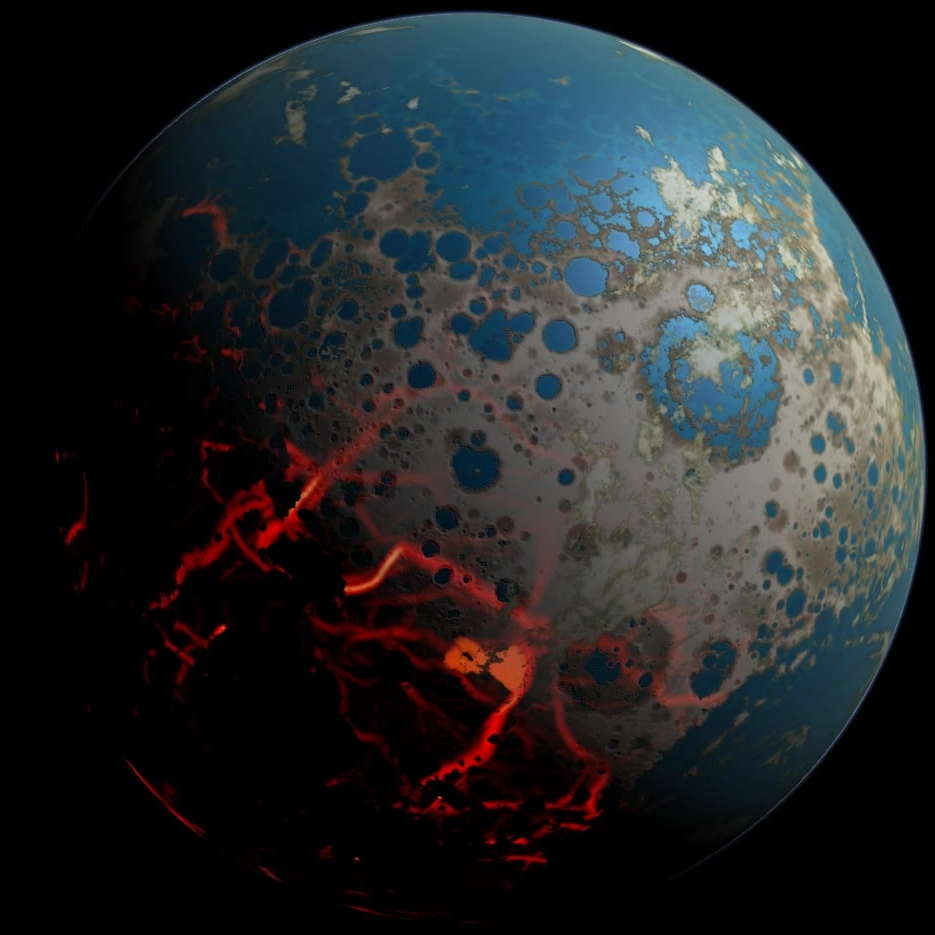
\includegraphics[width=0.7\textwidth]{early-earth.jpg}\EC
}

\frame{\frametitle{\textbf{Exam 3 grades}}
\Large
Some of you expressed a concern: students who had lab on Monday had an advantage on the exam.

\BS\pause

How can we determine if this is true?
}


{
\setbeamercolor{background canvas}{bg=white}
\frame{\frametitle{\textbf{Exam 3 grades}}
\BC
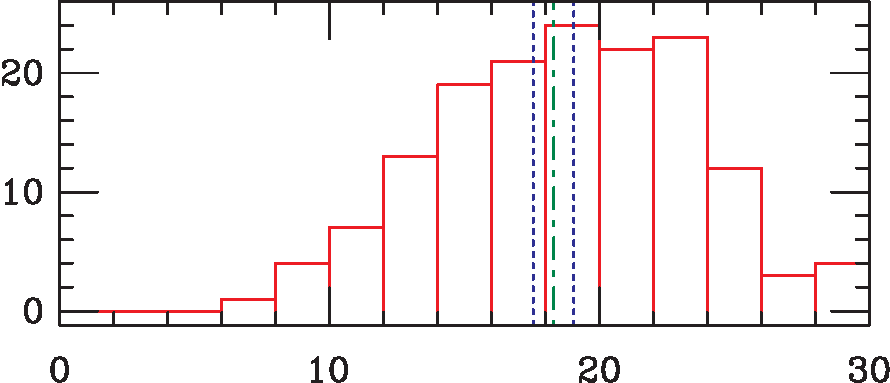
\includegraphics[width=0.7\textwidth]{earlyhisto-crop.pdf} \\
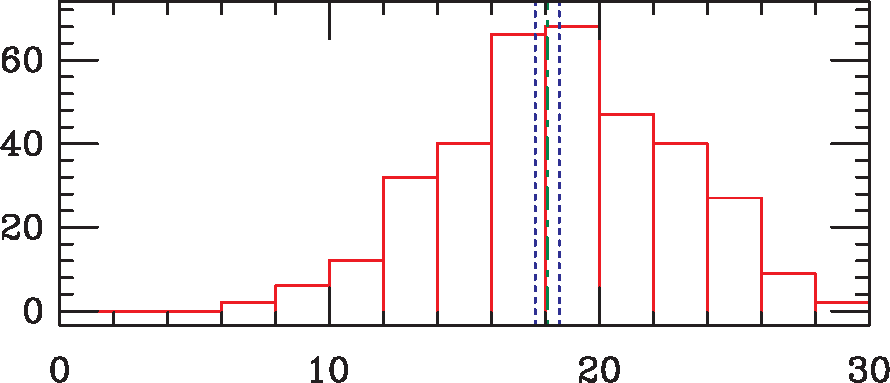
\includegraphics[width=0.7\textwidth]{latehisto-crop.pdf}

\BS

\pause
\EC
}
}

\frame{\frametitle{\textbf{Exam 3 grades}}
\Large
The difference was less than 1\%, well within the margin of error.

\BS\pause

However, it looks like there might be some effect on moderately-high scoring students. 

\BS

When I compare only those students scoring over 50\%, the averages differ by 2\%.

\BS\pause

I've decided to give everyone a one-point freebie -- essentially, scoring the exam out of 29 rather than 30.

}

\frame{\frametitle{\bf A spinning cloud of gas...}
\BC
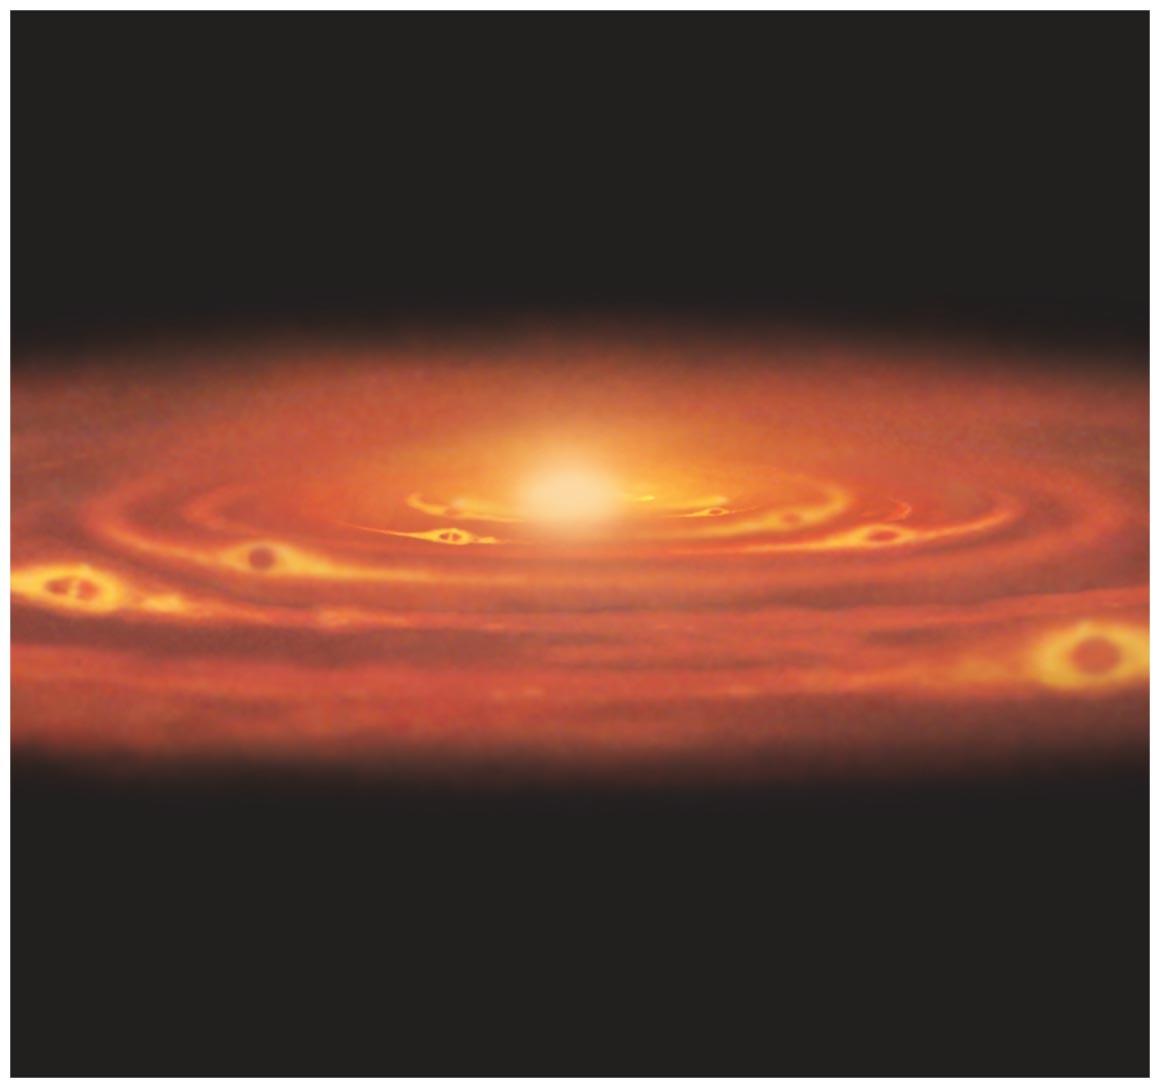
\includegraphics[width=0.5\textwidth]{ss-origin.jpg}
\EC

}

\frame{\frametitle{\bf ... bits coalesce into planets}
\BC
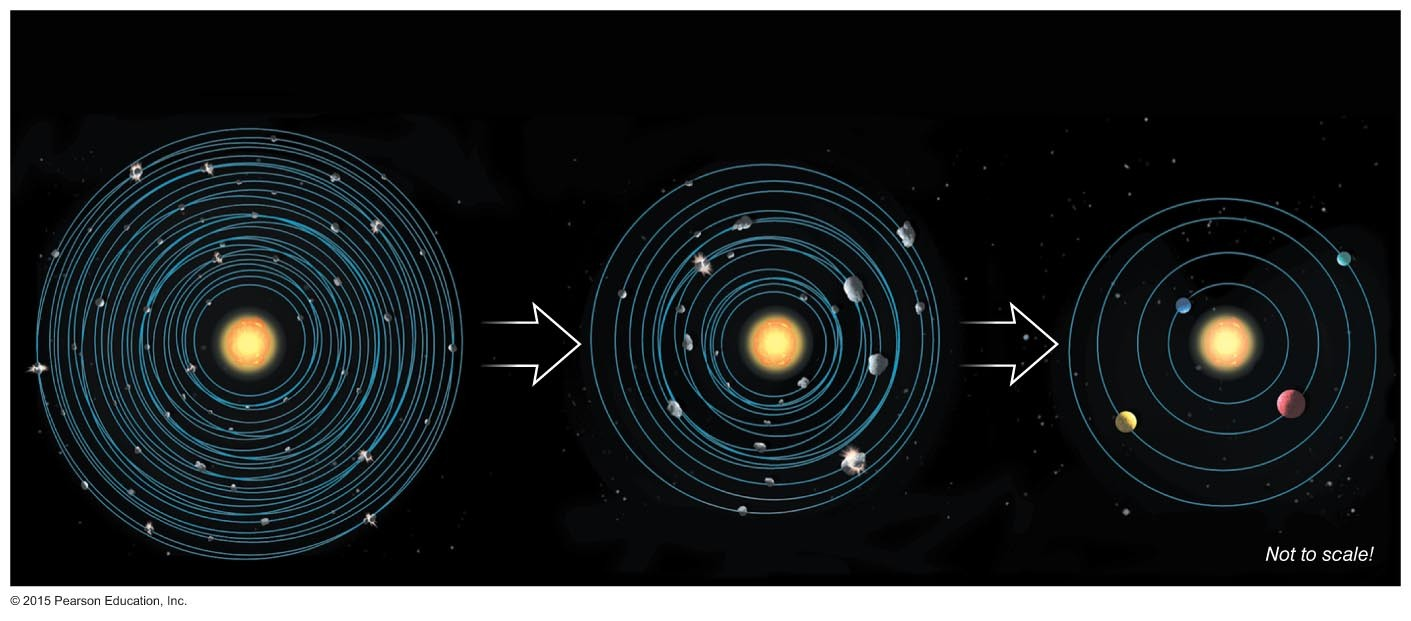
\includegraphics[width=0.8\textwidth]{planetesimals.jpg}
\EC
}

\frame{\frametitle{\bf The full picture}
\BC
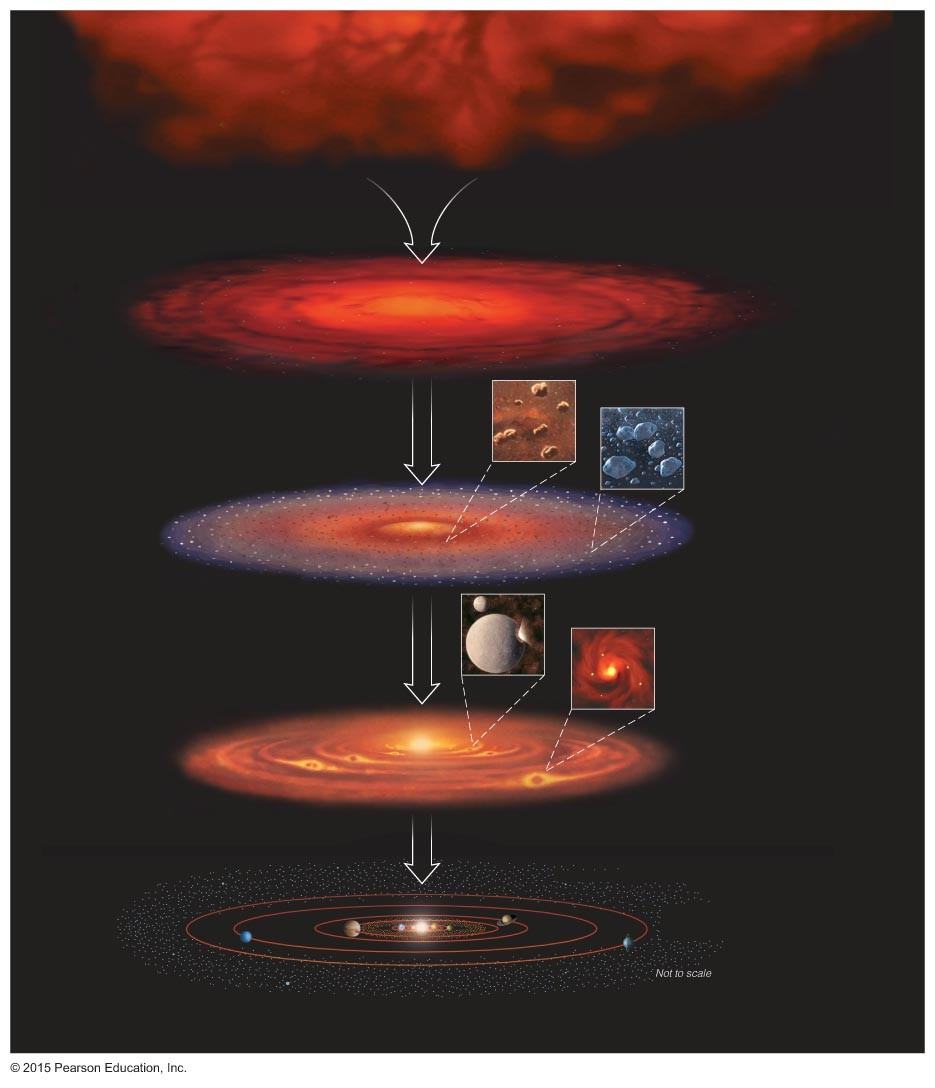
\includegraphics[width=0.5\textwidth]{ss-full-history.jpg}
\EC
}

\frame{

\huge

\BC
Complete {\it Lecture Tutorials} pp. 111-112.
\EC
}

\frame{\frametitle{\bf ... but how long ago was this?}

\large

The process used to figure out the ages of the planets is the same as the process used for more recent objects.

\BS\BS

``Carbon dating'': use the radioactive decay of carbon to figure out how old things are.

\BI
\item Useful for things up to about 50,000 years old
\EI

\BS\BS

We can use the decay of other isotopes to age much older things, though -- like planets!

}

\frame{
\BC
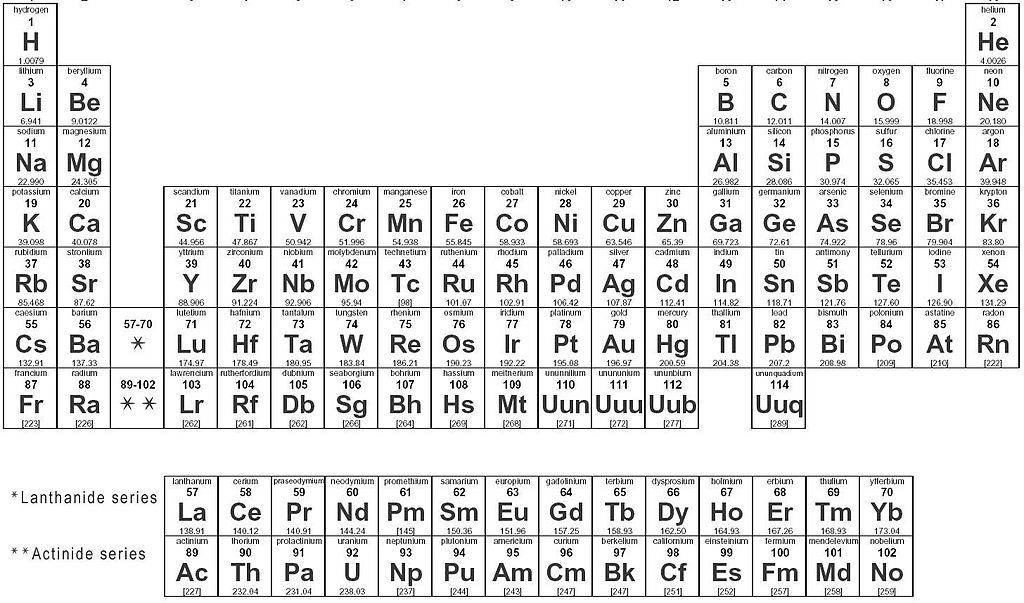
\includegraphics[width=0.95\textwidth]{periodic-table.jpg}
\EC
}

\frame{\frametitle{\bf Radioactive decay: key points}
\large
\BI
\item Each element on the periodic table has a fixed number of protons and electrons
\item The chemical properties don't depend on the number of neutrons
\item ``Ordinary'' carbon is called ``carbon-12''
\BI
\item It has six protons and six neutrons, for a total of twelve nucleons in the nucleus
\EI
\pause
\item A different form of carbon is called ``carbon-14''
\BI
\item It has six protons and eight neutrons, for a total of fourteen nucleons in the nucleus
\EI
\item These different forms of elements, with different numbers of neutrons, are called {\bf isotopes}
\EI
}



\frame{\frametitle{\bf Radioactive decay: key points}
\BI
\item Many isotopes are {\it radioactive}: they will decay into other isotopes of other elements after some time, eventually reaching a stable one
\item For instance: potassium-40 decays into argon-40; carbon-14 decays into nitrogen-14; uranium-235 decays (eventually) to lead-207
\item We can characterize how fast they decay by a number called the ``half-life''
\item One half-life: how long it takes for half of the substance to decay
\BI
\item ``Carbon-14 has a half-life of 5730 years''
\EI
\item We can use these decays as a clock
\EI
}

\frame{
\BS
\BC \large You give someone ten thousand pennies. Starting at noon, every hour she puts the pennies in a bucket and throws them on the floor, then removes all the ones that came up heads.



\BS
\BS

\Large You notice that at some point she has 2493 pennies left. About what time is it?

\EC
\color{A}A: 1:00 \\
\color{B}B: 1:30 \\
\color{C}C: 2:00 \\
\color{D}D: 2:30 \\
\color{E}E: 3:00 \\
\pause
\color{Orange}F: Please, please, don't make this a lab

}

\frame{
\large
\BI
\item Every hour half of her pennies come up heads and are removed
\pause
\item After one hour she'll have about 5,000 pennies left
\pause
\item After two hours she'll have about 2,500 pennies left
\pause
\item After three hours she'll have about 1,250 pennies left
\pause
\item $\rightarrow$ {\color{Red}Her pennies have a half-life of 1 hour}
\item The more pennies she started with, the more accurately I can tell time this way
\item There are {\bf far more} atoms in a sample than pennies here
\EI

\BS
\BC
Important difference with radioactive decay:
\EC
\BI
\item Radioisotopes don't decay every hour (or year or whatever); they decay continuously
\EI
}

\frame{\frametitle{\bf Radioactive decay: key points}
There aren't many of these unstable isotopes around, as you might expect.

\BS

\BI
\item Some of them, like carbon-14, are continually produced. 
\item Some of them, like uranium-235 and potassium-40, are left over from the supernova that produced them
\EI

\BS
\BS
\BC
{\color{Red}If we can figure out what fraction of the original amount of a radioisotope is left in an object, we can figure out how long ago it formed.}
\EC
}

\frame{\frametitle{\bf Carbon dating}
\large
Carbon-14 has a halflife of 5730 years and is continually produced in the atmosphere.

\BS

The fraction of carbon-14 in the atmosphere was historically nearly constant -- until recently. Why might that be?

\BS

\color{A}A: Explosion of nuclear weapons has increased the amount of radioactivity in the atmosphere \bigskip\\
\color{B}B: $\rm CO_2$ emissions from burning fossil fuels have added only carbon-12 to the atmosphere, not carbon-14 \BS\\
\color{C}C: The amount of cosmic rays hitting the atmosphere has changed because of the solar cycle \BS \\
\color{D}D: The metabolisms of plants and animals have changed with the rise of humans, absorbing carbon-12 but not carbon-14
}

{
\setbeamercolor{background canvas}{bg=white}
\frame{\frametitle{\color{Black}\bf Carbon dating}
\BC

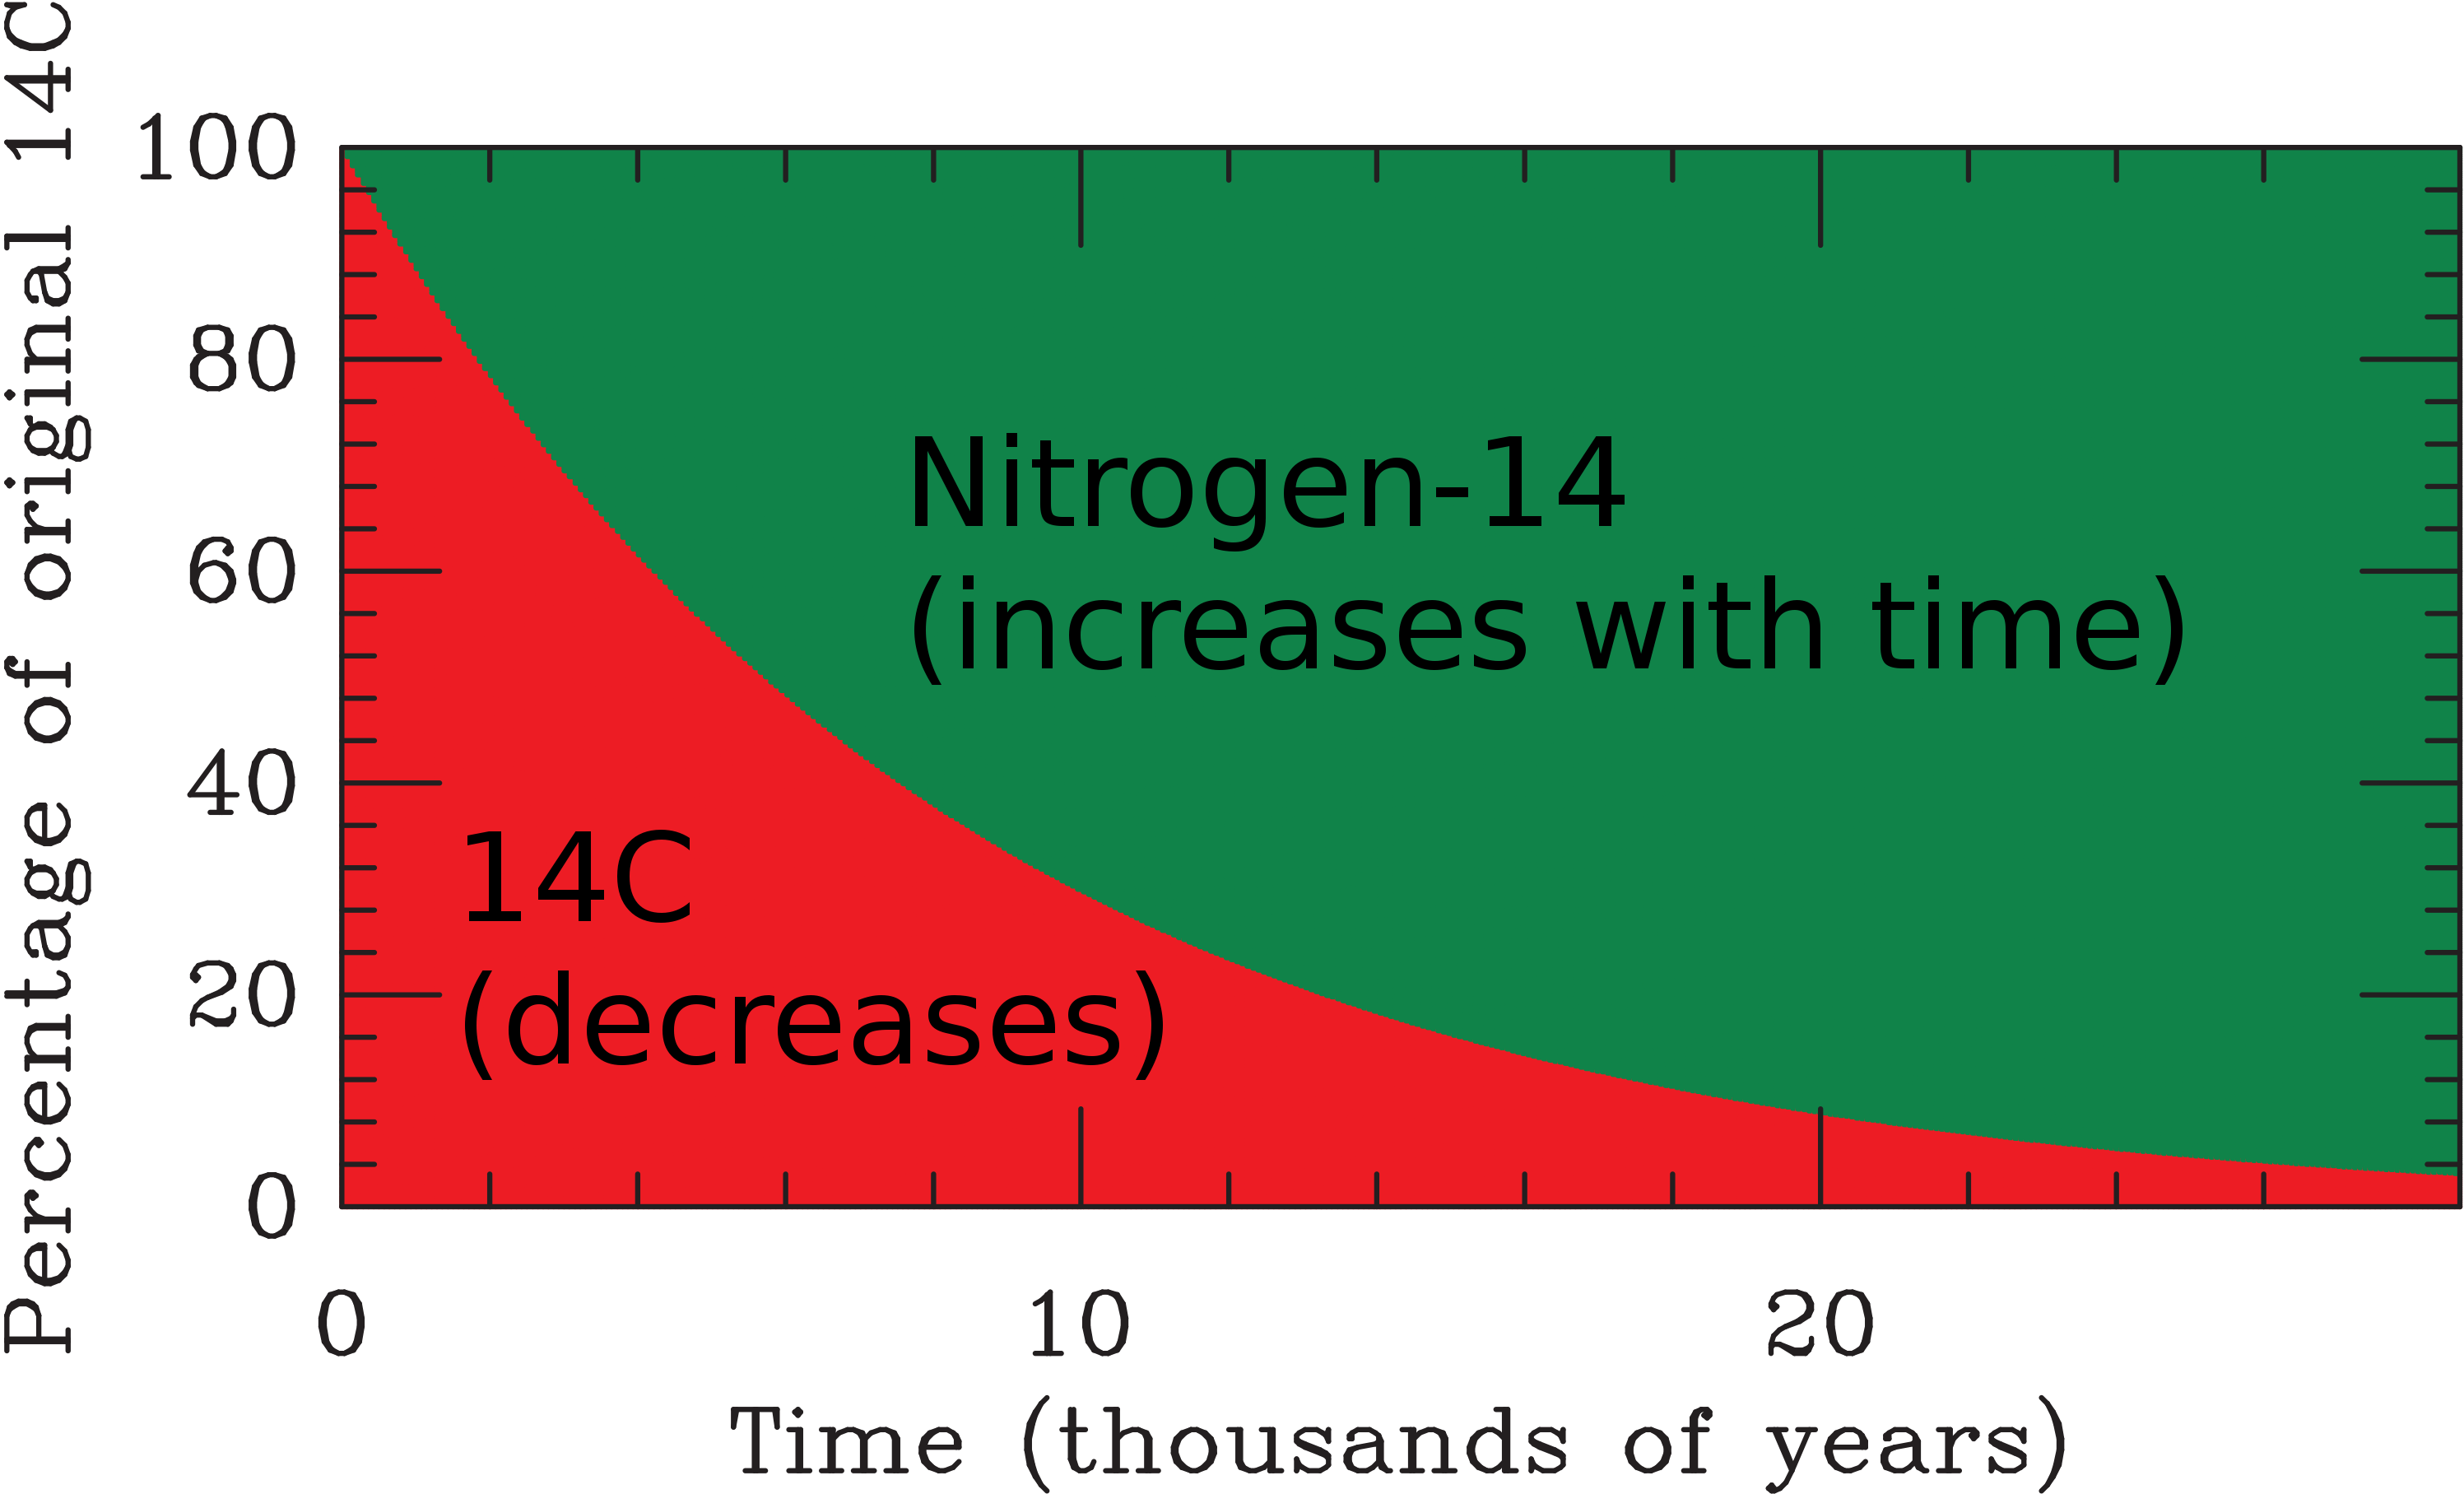
\includegraphics[width=0.65\textwidth]{carbon-fraction-crop.png}

\BS


\color{Black}
Living things constantly recycle their carbon, so their 14C fraction is the same as the atmosphere.

\BS

But once they die and stop breathing, over time 14C is replaced by 14N.

\BS

This lets us use the amount of 14C as a clock to see how long ago they died.
\EC
}
}
{
\setbeamercolor{background canvas}{bg=white}
\frame{\frametitle{\color{Black}\bf Carbon dating}
\BC

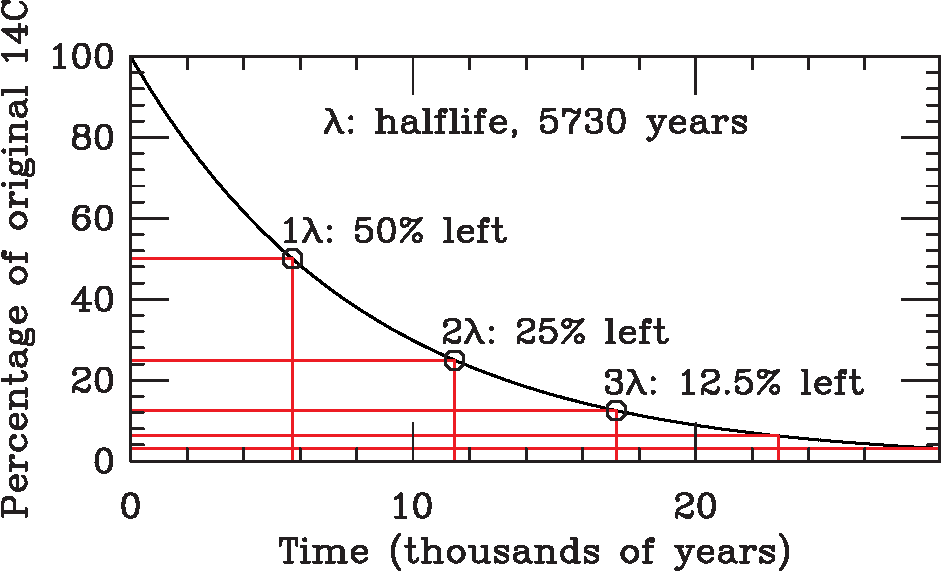
\includegraphics[width=0.65\textwidth]{c14-linear-crop.pdf}

\BS


\color{Black}
Living things constantly recycle their carbon, so their 14C fraction is the same as the atmosphere.

\BS

But once they die and stop breathing, over time 14C is replaced by 14N.

\BS

This lets us use the amount of 14C as a clock to see how long ago they died.
\EC
}
}
{
\setbeamercolor{background canvas}{bg=white}
\frame{\frametitle{\color{Black}\bf Carbon dating}
\BC

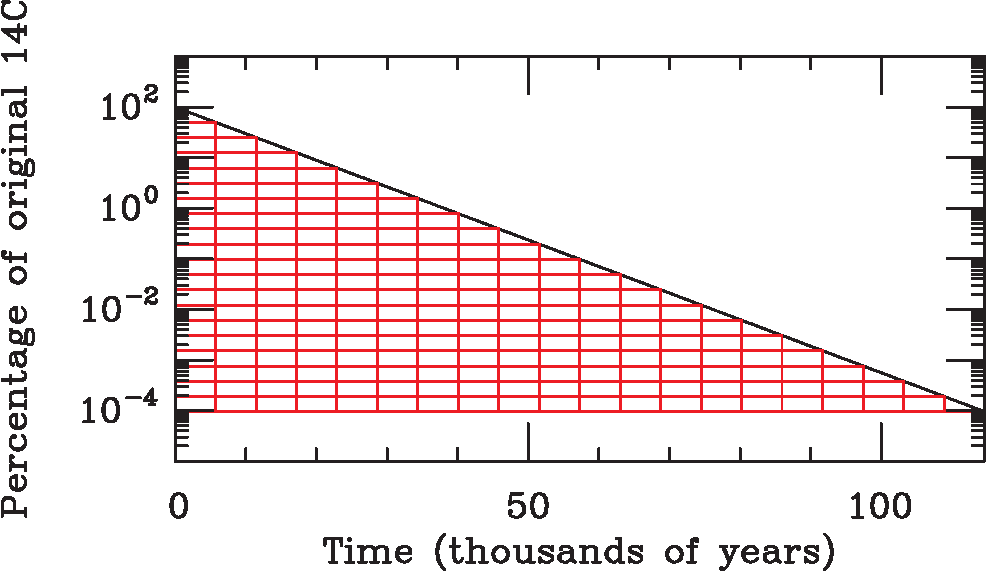
\includegraphics[width=0.65\textwidth]{c14-log-crop.pdf}

\BS


\color{Black}
We can use this procedure on things up to about 50,000 years old.

\BS

Past that, the 14C fraction is too small to give an accurate picture.

\BS

We need some older process to date the planets!
\EC
}

\frame{\frametitle{\color{Black}\bf Other radioisotopes}
\large
\color{Black}
There are longer-lived isotopes we can use here:

\BI
\color{Black}
\item Potassium-40: half-life of 1.251 Gyr (``gigayears'' -- billion years). Decays into argon-40.
\item Uranium-235: half-life of 0.7038 Gyr. Decays into lead-207.
\EI

This radioactive decay works the same way:

\BC
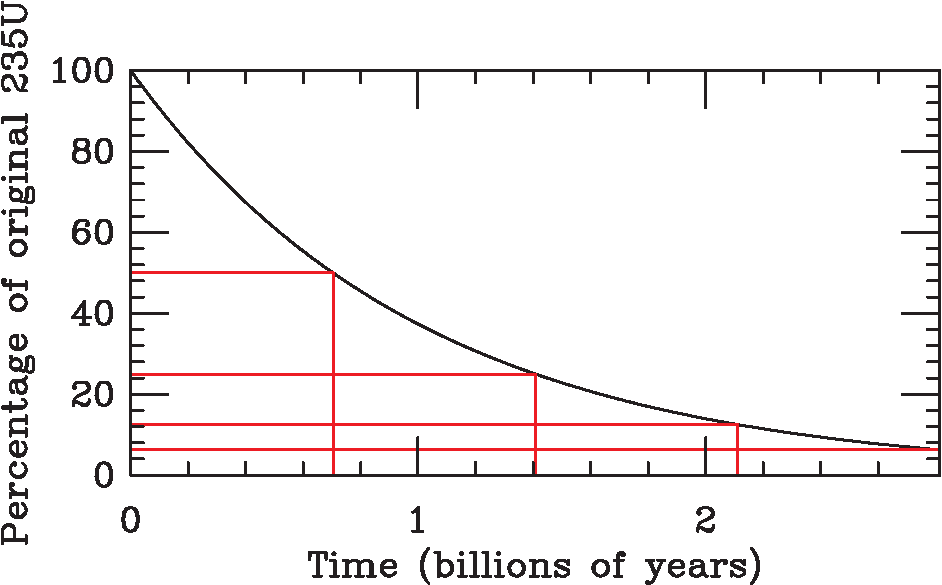
\includegraphics[width=0.45\textwidth]{u235-lin-crop.pdf}
\hspace{0.08\textwidth}
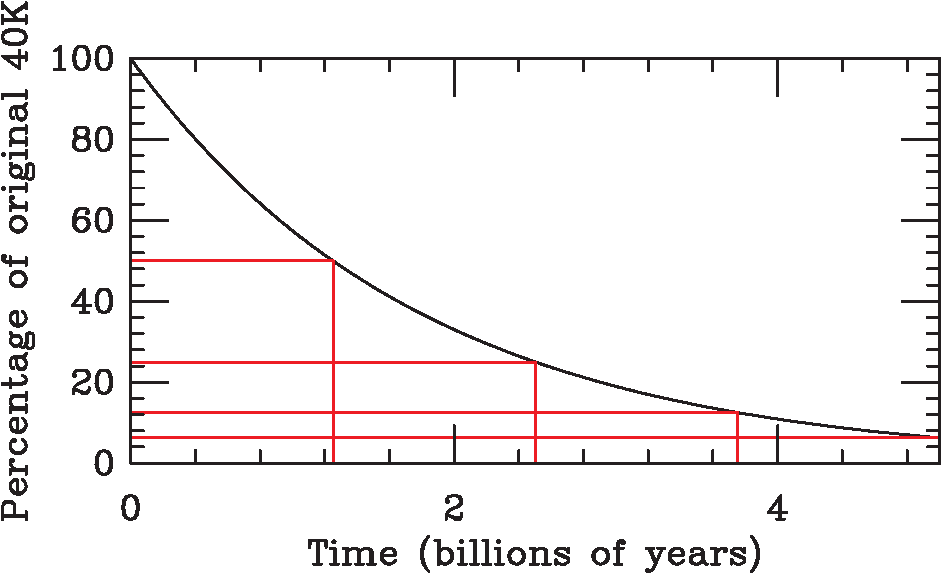
\includegraphics[width=0.45\textwidth]{k40-lin-crop.pdf}
\EC
}

}

\frame{\frametitle{\bf Uranium-lead dating}

\large

Crystals of the mineral zircon readily incorporate uranium into their structure, but {\it not} lead, while they are forming.

\BS

Thus any lead present in zircon got there through the decay of uranium-235.

\pause
\BS
\BS
A zircon crystal contains as many atoms of lead-207 as uranium-235. About how old is it? (The halflife of U-235 is about 0.7 billion years.)

\Large
\BS
\color{A}A: 0.7 Gyr\\
\color{B}B: 1.4 Gyr\\
\color{C}C: 2.1 Gyr\\
\color{D}D: 2.8 Gyr
}


\frame{\frametitle{\bf Uranium-lead dating}

\large

Crystals of the mineral zircon readily incorporate uranium into their structure, but {\it not} lead, while they are forming.

\BS

Thus any lead present in zircon got there through the decay of uranium-235.

\pause
\BS
\BS
A zircon crystal contains seven atoms of lead-207 for every atom of uranium-235. About how old is it? (The halflife of U-235 is about 0.7 billion years.)

\Large
\BS
\color{A}A: 0.7 Gyr\\
\color{B}B: 2.1 Gyr\\
\color{C}C: 4.9 Gyr\\
\color{D}D: 5.6 Gyr
}

\frame{\frametitle{\bf Potassium-argon dating}

\large

Argon is a noble gas. It doesn't chemically bond readily.
\BS

Thus any argon-40 present in zircon got there through the decay of potassium-40. Potassium-40 has a half-life of about 1.251 Gyr.

\BS
\BS

These two processes -- lead/uranium dating and potassium/argon dating -- rely on different assumptions, so they are a nice crosscheck.
}

\frame{\frametitle{\bf Now, let's date some rocks!}
\pause
\BC
(no, not like that)
\EC

\large
\BI
\item Oldest Earth rocks: 4 Gyr (a few grains are a bit older)
\item Oldest Moon rocks: 4.4 Gyr
\item ... can we get anything older than that? What are the most primordial things in the Solar System?
\EI
}

\frame{\frametitle{\bf Now, let's date some rocks!}
\BC
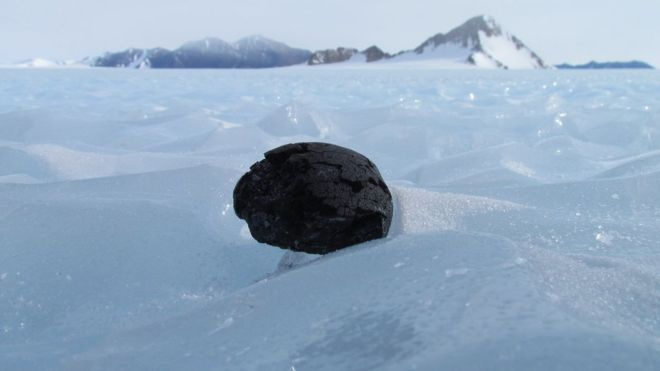
\includegraphics[width=0.6\textwidth]{meteorite.jpg}


\BS

Some meteorites found on Earth date to 4.55 Gyr old -- the age of the condensation of the first rocks in the Solar System.

\EC
}

\frame{\frametitle{\bf What about other planets?}

\url{https://www.caltech.edu/news/first-rock-dating-experiment-performed-mars-41496}

We've done argon/potassium dating on Mars, giving the same results as Earth: a bit more than four billion years.
}


\end{document} 
